\chapter{Work Done}\label{C:workdone}
The work currently accomplished within the project can be seen in the subsections below:
\subsection{Technical Work}
\subsubsection{Technologies Chosen}
The technologies chosen for this project are: a jQuery frontend application, with a node.js/socket server using mongoDB as a datastore within the application. 
\begin{itemize}
\item \textbf{jQuery:} \cite{js.foundation_2018}  This was chosen as the front-end framework for the application on the advisement of my project supervisor. This is due to the current technologies that are housed within the aWall application. jQuery was one of the technologies that was picked that is currently housed within the overall aWall prototype, allowing for simple integration between the two software prototypes. 
\item \textbf{Node.js:} \cite{foundation_2018} Node.js was chosen as the backend framework due to its ability to quickly setup and integrating into other parts of the prototype through libraries such as \textit{Socket.IO} \cite{socket.io_2018} for Sockets and \textit{Mongoose} \cite{mongoose-odm-v5.1.3_2018} for MongoDB. The aWall prototype does not use Node.js as a technology, its backend framework is \textit{Python} \cite{welcome-to-python.org_2018}, this wasn't chosen due to the complexity of integration with the other technologies. 
\item \textbf{Sockets:} \cite{socket.io_2018} Sockets were needed for this project due to the need of real-time communication within the prototype between the participant and screen systems. This was chosen due to it being one of the technologies within the current aWall prototype, therefore making it easier to integrate the two prototypes together.
\item \textbf{MongoDB:} \cite{mongodb-for-giant-ideas_2018} MongoDB was chosen as the datastore for the prototype, this is not the datastore held within the current aWall project, as that datastore will not allow me to store the correct data needed for the retrospective section. \textit{MongoDB}, more specifically \textit{MongoAtlas} \cite{fully-managed-mongodb-hosted-on-aws-azure-and-gcp_2018} was chosen due to it's simplicity and quickness to setup and get something running. It also allows for easy integration within the backend framework with the library \textit{Mongoose} \cite{mongoose-odm-v5.1.3_2018}.
\end{itemize}
With using both jQuery and Socket.IO as the major libraries within the frontend development of the application it has made it possible to very easily slip out the backend that has been developed within this prototype and integrate this frontend into the current prototype of aWall that uses both of these technologies with minimal change.

\subsubsection{Design}
The current design of the prototype can been seen below:
\begin{figure}[ht]
\centering

\includegraphics{placeholder}
\caption{Current Design Framework of aWall Retrospective Prototype}
\end{figure}
\\
As we can see from the picture in Figure 2, the participate and screen systems have direct links to server through both the sockets and through requests. The need for the socket connections to go through the server is useful for data store and manipulation before being send out, allowing for more calculation and processing strain on the server rather than the users device. 
The need for both the socket communication and requests between the server and other systems is due to the need for joining and create retrospective boards within the system. The sockets are stored within a map on the server, with needing a name that is given on joining a session to properly store the data. Therefore due to this, the need for requests is required to send data when joining a session.

The connection between the database, sockets and the server is setup during the startup of the server and remains open and available during the entire time the server is alive.
\subsubsection{Current Implementation Progress}
The current implementation progress within this system is as follows:
\begin{itemize}
\item \textbf{Server:} The server has been fully setup with its socket counterpart and its connection to the datastore MongoDB. It currently has built within it a framework that allows for easy ability to add and remove extra retrospectives within itself, with 3 of the 6 retrospective types having this completed. The server is also being current hosted within the ECS system at Victoria University and can be found at: \url{http://barretts.ecs.vuw.ac.nz:52724/}
\item \textbf{Screen:} Within the screen system, the header component with its required scope file working and also one of the retrospective methods. This header file is constant throughout the entire retrospective for the screen, it displays the most important data throughout the entire retrospective such as time elapsed, members and current stage. The work for the first retrospective type, Check-in has also been completed, with connection to the server to grab the required data for it. 
\begin{figure}[ht]
\centering
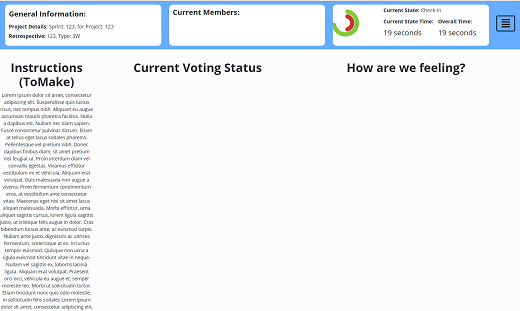
\includegraphics{moderator_progress}
\caption{Current Progress of Screen System within aWall Retrospective Prototype}
\end{figure}
\item \textbf{Participant:} The participant view, the only progress that has been made has been within it has been the voting system for the first retrospective and the connection to server to write the data to the datastore.
\begin{figure}[ht]
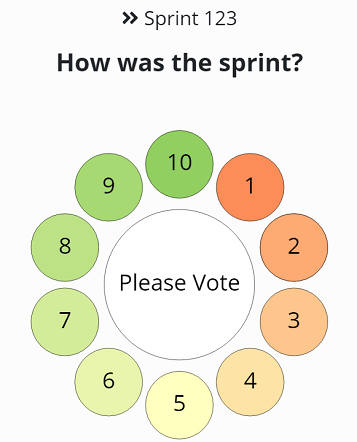
\includegraphics{participant_progress}
\centering
\caption{Current Progress of Participant System within aWall Retrospective Prototype}
\end{figure}
\end{itemize}
